
\chapter{Gerarchia delle memorie, più a fondo}
\label{cha:gerarchiaDettagli}

\section{La gerarchia e le sue peculiarità}
\label{sec:gerarchiaPeculiarità}

In questo capitolo andremo più a fondo nella questione riguardante la gerarchia delle memorie. Fin'ora abbiamo capito che:
\begin{itemize}
\item la \textit{cache} è una memoria piccola e molto costosa, ma estremamente veloce;
\item la memoria centrale è interconnessa al bus esterno della CPU ed è mappata nello spazio di indirizzamento in memoria;
\item la memoria virtuale è quella vista dal sistema operativo; si trova su un supporto di memorizzazione esterno ed è indirizzabile come una periferica;
\item i segmenti sono visti dalle applicazioni (e anche dal sistema operativo): la protezione tra programmi può
essere realizzata organizzando lo spazio di indirizzamento logico in segmenti
protetti.
\end{itemize}
Mentre i blocchi a livello di memoria segmentata possono avere qualunque dimensione, gli altri livelli sono tutti a dimensione costante (le pagine sono sempre di 4 KB, le linee di \textit{cache} sempre di 32 byte, etc\ldots).

\begin{figure}[!h]
\centering
\includegraphics[width=\columnwidth]{img/gerarchiamemorie}
\caption{Gerarchia delle memorie}
\label{fig:gerarchiamemorie}
\end{figure}

In un sistema in cui la memoria è organizzata in una gerarchia di livelli, il funzionamento è il seguente: la CPU cerca l'informazione nel livello più vicino e, se la trova, la utilizza. In caso contrario la cerca nel livello immediatamente successivo; se lì è presente, copia un blocco di memoria contenente l'informazione desiderata nel livello precedente, quindi la cerca di nuovo nel livello più vicino. Se non la trova ancora, la cerca nel livello ancora successivo, quindi torna al punto precedente.

Il trasferimento di un blocco da un livello al livello adiacente viene effettuato secondo modalità che dipendono dalla velocità dei supporti di memoria associati ai livelli coinvolti Viene effettuato dal sistema operativo nel caso il tempo di accesso al livello corrente sia compatibile col tempo di esecuzione di una procedura (ad esempio in memoria virtuale o in memoria fisica). Viene effettuato dall'\textit{hardware} in modo trasparente a tutto il
software incluso il S.O., se l'\textit{overhead} introdotto da una gestione software avesse sul tempo di accesso medio l'effetto di annullare il vantaggio ottenibile dall'introduzione della memoria più veloce (ad esempio la \textit{cache}).

%\begin{figure}[!h]
%\centering
%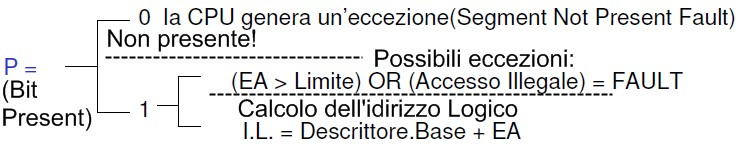
\includegraphics[width=0.75\columnwidth]{img/bitPresent}
%\caption{Il bit \textit{Present} e traduzione}
%\label{fig:bitPresent}
%\end{figure}

Perché tutta la baracca stia in piedi, a ogni livello e a ogni blocco deve essere associato un descrittore che deve dire se il blocco è presente o meno (bit \textit{Present}) (e in entrambi i casi suggerisce come reperirlo): in caso positivo il descrittore contiene l'indirizzo del blocco, altrimenti deve indicare come reperirlo. I descrittori delle pagine stanno nella PTE (\textit{Page Table Entry}) e hanno dimensione pari a 4 byte. Le informazioni in essi contenute sono più o meno quelle dei descrittori già visti nei precedenti capitoli. 

\section{Spazio dei segmenti}
\label{sec:segmentiSpace}

L'IA32 ha come caratteristica l'organizzazione segmentata della memoria vista dal programmatore assembler (spazio di indirizzamento logico). A ogni segmento è associato un descrittore di 8 byte contenente tutte le
caratteristiche del segmento stesso. I descrittori sono riuniti in due tabelle chiamate \textit{tabelle dei descrittori} o più precisamente GDT (\textit{Global Descriptor Table}) e LDT (\textit{Local Descriptor Table}). Ai descrittori si accede mediante un selettori da 16 bit e contenete sia le informazioni riguardanti la tabella d'appartenenza (GDT o LDT), sia l'indice del descrittore nella tabella.

\begin{figure}[!h]
\centering
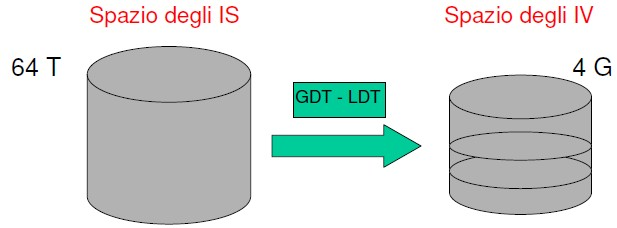
\includegraphics[width=0.65\columnwidth]{img/segmentiVirtuale}
\caption{Da spazio dei segmenti a memoria virtuale}
\label{fig:segmentiVirtuale}
\end{figure}

Visto che la memoria logica (spazio dei segmenti) è di 64 TB, mentre lo spazio di indirizzamento della memoria virtuale è di 4 GB, come si può passare da un livello all'altro? Quando la CPU ha bisogno di un nuovo oggetto ma la memoria a livello inferiore è satura, c'è bisogno di sostituire degli oggetti utilizzati poco recentemente con gli oggetti richiesti (sostituzione, della quale si occuperà un particolare algoritmo in grado di rispettare il principio di località, etc\ldots). Lo spazio logico da 64 TB viene mappato sullo spazio degli indirizzi virtuali e non sulla memoria fisica per lasciare al software uno spazio di 4 GB disponibile senza pericolo di "'\textit{segment non present fault}'", indipendentemente dalla dimensione della memoria fisica (che spesso è più piccola di 4 GB e non potrebbe magari contenere tutto il codice). 

\section{Memoria virtuale}
\label{sec:memoriaVirtuale}

Lo spazio di indirizzamento virtuale è uno spazio di indirizzamento la cui dimensione è indipendente dalla dimensione della memoria fisica accessibile. Il principale obiettivo del sistema di memoria virtuale è utilizzare al
meglio la memoria fisica disponibile in modo trasparente al programmatore (che non si deve preoccupare della dimensione del proprio codice, né stare a impazzire con strane traduzioni degli indirizzi), sfruttando il principio di località e appoggiandosi a una memoria di massa ausiliaria (tipicamente l'\textit{Hard Disk}). Il principio di funzionamento è quindi il seguente: gli oggetti già utilizzati dalla CPU stanno in memoria centrale (RAM), mentre i nuovi oggetti richiesti dalla CPU vengono richiamati dal disco (memoria virtuale) e vanno a rimpiazzare in memoria centrale gli oggetti utilizzati meno recentemente. Risulta dunque necessario partizionare i programmi in blocchi ciascuno dei quali viene richiamato in memoria solo quando serve.

Mentre la dimensione dei segmenti possiamo deciderla noi spaciugando nel relativo descrittore, i quattro gigabyte di memoria virtuale sono divisi in pagine tutte uguali e di dimensione fissa (4 KB). Nella tabella dei descrittori di queste pagine (\textit{Page Table}) possono starci quindi fino a 1 Mega \textit{entries} ($4 KB \cdot 1 M = 4 GB$).

Per consentire alla CPU l'accesso alla memoria fisica è necessario trasformare l'indirizzo logico in indirizzo fisico. Siccome la memoria virtuale è suddivisa in pagine di uguale dimensione, e dato che quest'ultima (4 KB) è uguale a quella delle pagine in memoria fisica, passare all'indirizzo fisico a partire dall'indirizzo lineare (cioè in memoria virtuale) è davvero elementare. Supponiamo di avere un dato di nome PIPPO, mappato a
\begin{verbatim}
MEMORIA VIRTUALE -> IV(PIPPO) = 32D0 (n° pagina da 4KB = 3; offset = 2D0)
MEMORIA FISICA   -> IF(PIPPO) = 12D0 (n° pagina da 4KB = 1; offset = 2D0)
\end{verbatim}
Come si vede, l'uguale dimensione delle pagine in memoria fisica e in memoria virtuale permette di mantenere inalterato l'offset\footnote{Le quantità nell'esempio sono esadecimali. La cifra più significativa del numero della pagina è chiaramente il 12° bit, visto che $2^12 =4K$, quindi trovare l'offset e il \textit{Page ID} è facilissimo: il primo consiste nelle tre cifre esadecimali meno significative, mentre quelle più significative formano il numero della pagina.} nella pagina da 4 KB. Quel che cambia, fra le due memorie, è il numero della pagina: nel primo caso il \textit{page ID} sarà 3, nel secondo 1. Dunque è necessario conoscere l'identificatore della pagina per poterla trasferire dall'una all'altra memoria: l'offset, invece, si conserva e basta quindi copiarlo inalterato nel passaggio.

\begin{figure}[!h]
\centering
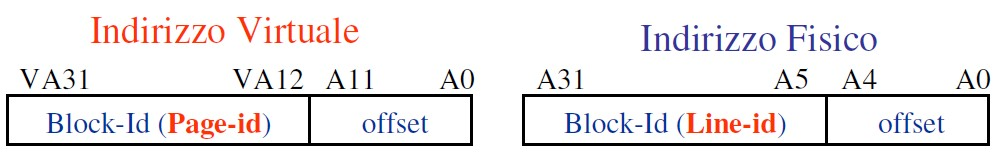
\includegraphics[width=0.75\columnwidth]{img/ivif}
\caption{Da indirizzo virtuale a indirizzo fisico}
\label{fig:ivif}
\end{figure}

La struttura nella quale viene memorizzata la corrispondenza fra gli ID delle pagine è la \textit{Page Directory}, come mostrato in figura \ref{fig:memoriaVirtFis}.

\begin{figure}[!h]
\centering
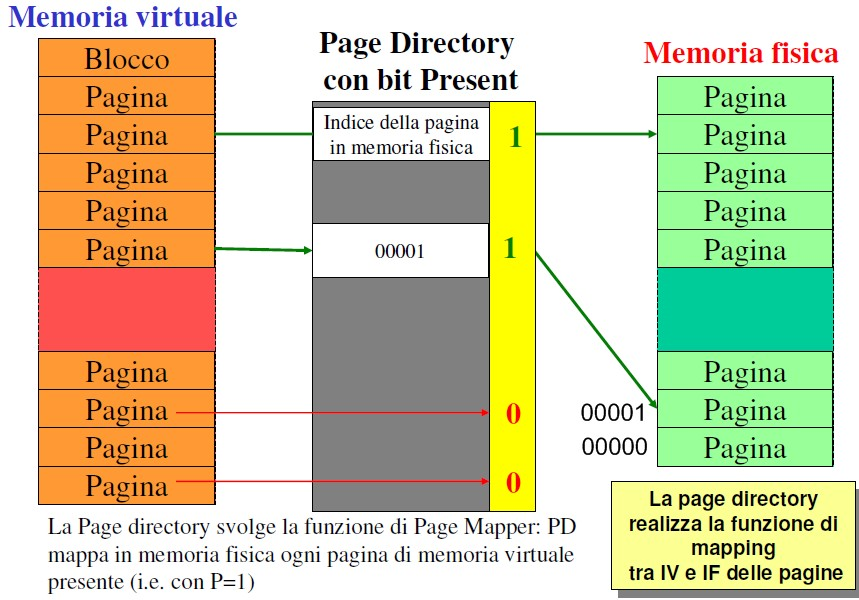
\includegraphics[width=0.85\columnwidth]{img/memoriaVirtFis}
\caption{L'utilità della \textit{Page Directory}}
\label{fig:memoriaVirtFis}
\end{figure}

Questa traduzione avviene nella fase AG e richiede due cicli di bus: uno alla tabella, per poter capire quale sia l'ID giusto, e l'altro all'operando. Se il bit \textit{Present} è pari a 0, dobbiamo invece gestire un particolare tipo di \textit{miss} denominato \textit{page fault} (manca la pagina: dobbiamo andarla a pescare nello spazio dei segmenti).

In figura \ref{fig:indirizzamento} possiamo osservare il meccanismo di traduzione degli indirizzi da memoria segmentata a memoria virtuale e infine a memoria fisica. Si noti che il calcolo in memoria virtuale viene effettuato tramite una somma, mentre quello in memoria fisica viene fatto più velocemente tramite un concatenamento (vedi fig. \ref{fig:sommaVSconcatenamento}).
\begin{itemize}
\item l'indirizzo nello spazio segmentato (IS) viene calcolato utilizzando l'indirizzo del selettore e il registro EA (16 bit di EAX);
\item l'indirizzo nello spazio virtuale viene ottenuto tramite somma di base e EA;
\item l'indirizzo nello spazio fisico viene ottenuto concatenando al corretto ID della pagina l'offset costituente le 12 cifre meno significative di IV. 
\end{itemize}

\begin{figure}[!h]
\centering
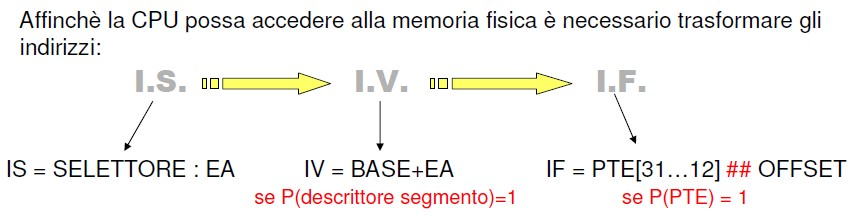
\includegraphics[width=0.85\columnwidth]{img/indirizzamento}
\caption{Schema di traduzione degli indirizzi}
\label{fig:indirizzamento}
\end{figure}

\begin{figure}[!h]
\centering
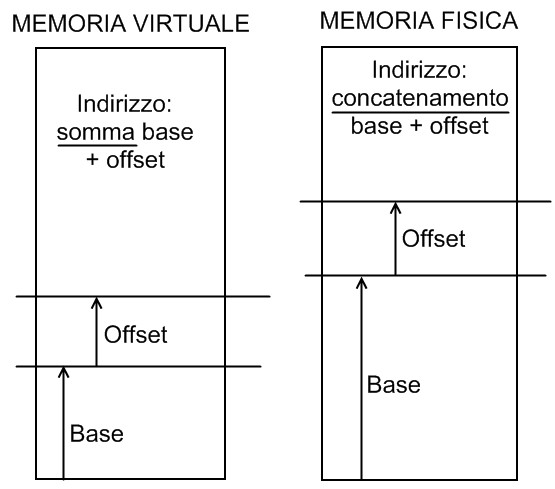
\includegraphics[width=0.45\columnwidth]{img/sommaVSconcatenamento}
\caption{Somma vs. concatenamento}
\label{fig:sommaVSconcatenamento}
\end{figure}

\clearpage

\subsection{Registro CR3 e tabelle}
\label{sec:CR3}

La \textit{page directory} con bit \textit{Present} è puntata dal registro CR3 della CPU, per cui lo schema di traduzione è quello in figura \ref{fig:belvaCR3} (\textit{mapping a un livello}).

\begin{figure}[!h]
\centering
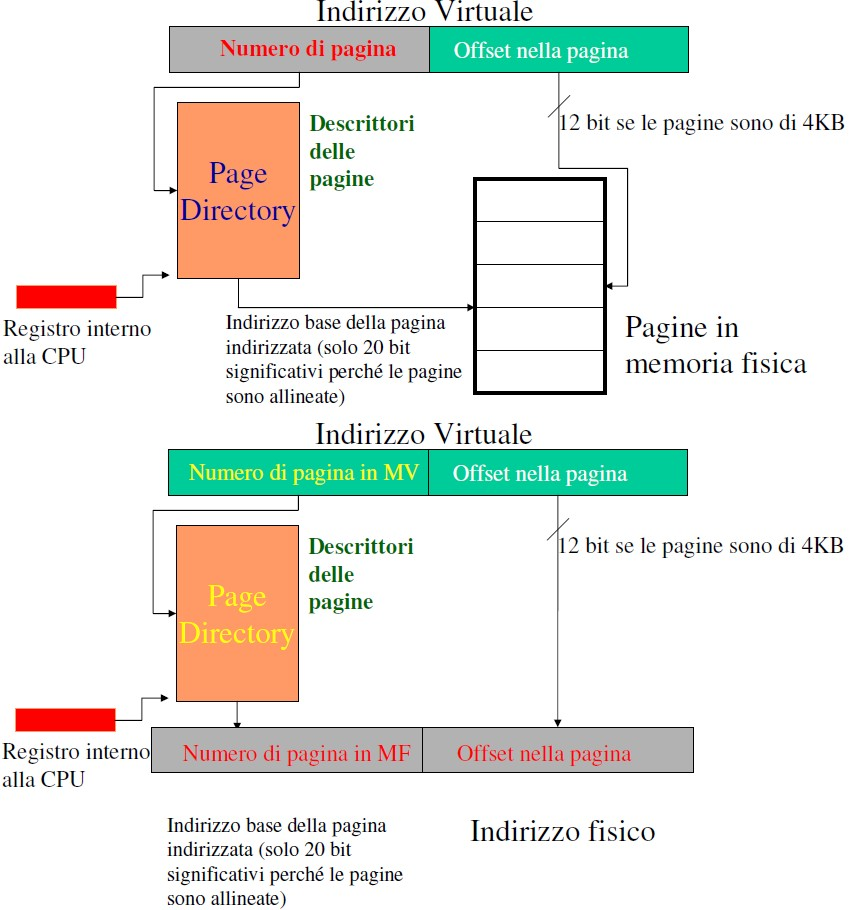
\includegraphics[width=0.86\columnwidth]{img/belvaCR3}
\caption{Trasformazione IV $\to$ IF: \textit{Address Mapper} a un livello}
\label{fig:belvaCR3}
\end{figure}

L'indirizzo virtuale, nel nostro Pentium, è tuttavia diviso in tre parti (\textit{mapping a due livelli}), come si può vendere in figura \ref{fig:3parti}.

\begin{figure}[!h]
\centering
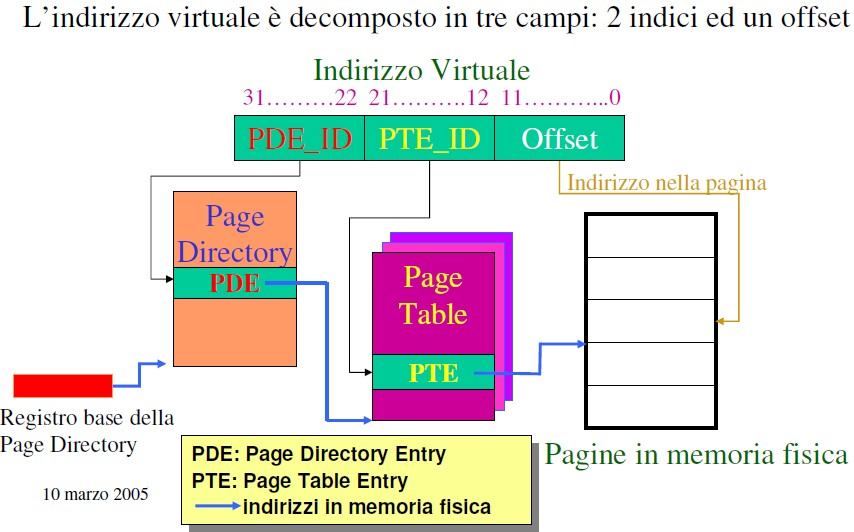
\includegraphics[width=0.87\columnwidth]{img/3parti}
\caption{Trasformazione IV $\to$ IF: mapping a due livelli}
\label{fig:3parti}
\end{figure}

Il primo indice (PDE\_ID, \textit{Page Directory Entry ID}) è l'ID della "'riga'" (cioè della \textit{entry}) della \textit{Page Directory}: la nostra PD, grande 4 KB, contiene infatti 1 K \textit{entries} da 4 byte ognuna delle quali conserva al suo interno l'indirizzo di una certa \textit{Page Table}. Il secondo indice (PTE\_ID, \textit{Page Table Entry ID}) discrimina fra le $2^{10} = 1 ~K$ possibili \textit{entry} di una delle $2^{10} = 1 ~K$ possibili \textit{Page Table} selezionabili tramite 10 bit MSB. Ogni PT contiene 1 K \textit{entry}, ognuna delle quali si riferisce ad una pagina di 4 KB ($2^{12}$ byte): per questo gli ultimi 12 byte sono l'offset all'interno della pagina selezionata dalla PTE.

Vantaggi di questo approccio (\textit{mapping a due livelli}):
\begin{itemize}
\item la PD (residente in memoria) è piccola;
\item le PT risiedono in generale nella Memoria di massa e vengono richiamate in Memoria centrale solo all'occorrenza.
\end{itemize}
Svantaggio di tale approccio: per determinare l'indirizzo fisico obiettivo sono necessari due accessi in memoria.

\begin{figure}[!h]
\centering
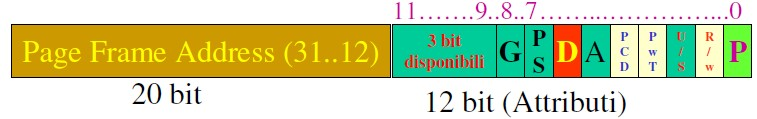
\includegraphics[width=0.75\columnwidth]{img/ptepde}
\caption{Formato dei descrittori delle PTE e delle PDE}
\label{fig:ptepde}
\end{figure}

In figura \ref{fig:ptepde} possiamo vedere il formato dei descrittori di PTE e PDE:
\begin{itemize}
\item P: presente (in memoria fisica);
\item R/W: protezione sulla pagina (1 = \textit{write enable});
\item U/S: autorizzazione all'accesso (U: \textit{user} - S: \textit{supervisor level});
\item PWT: politica di scrittura in \textit{cache} (viene utilizzato anche per segnalare alla \textit{cache}
di secondo livello che la \textit{cache} di primo livello è \textit{write-through});
\item PCD: \textit{cache disable};
\item A: settato ad ogni accesso alla pagina, sia in lettura, sia in scrittura (\textit{accessed});
\item D: settato ad ogni scrittura sulla pagina (\textit{dirty}). Il bit ha significato solo se la
PDE o PTE punta a una pagina, se no vale zero;
\item PS (\textit{page size}), solo nelle PDE, indica se la pagina è da 4 KB o da 4 MB;
\item G (\textit{global}) indica che una pagina in memoria è globale, per cui non viene invalidata
nel TLB quando si aggiorna CR3 o quando c'è una commutazione di \textit{task}.
\end{itemize}

Quando la CPU deve eseguire una trasformazione IV/IF accede alla PT desiderata tramite PDBR (\textit{Page Directory Base Register}) e PD; gli indirizzi contenuti in PDBR, PD e PT sono indirizzi fisici: dunque, in questa situazione, PD e PT sono mappate in memoria fisica. Quando invece il gestore della memoria virtuale (il SO) deve aggiornare PD e PT, accede ad esse tramite il software, ma gli operandi sono mappati in memoria virtuale; dunque in questa situazione PD e PT vengono viste in memoria virtuale e gli indirizzi contenuti in PD sono interpretati come
indirizzi virtuali. Quindi per evitare incongruenze tra SO e CPU è necessario che IV e IF di \textit{Page Directory} e \textit{Page Tables} siano identici (\textit{Mapping} Identico).

\section{Memoria fisica}
\label{sec:memFisica}

Il sistema operativo, per poter effettuare un efficiente trasferimento delle pagine tra MV e MF conserva una propria \textit{free-list} per sapere quali blocchi siano liberi in memoria fisica. Chiaramente, se essa è piena, è necessario cancellare una pagina poco utilizzata: per capire quale pagina possa fare a tale nostro scopo, ad ogni oggetto si affianca un particolare bit (A) che viene posto ad 1 quando si accede a tale oggetto. Chiaramente, a priori, A sarà uguale ad 1 (ho appena trasferito la pagina), tuttavia un timer, dopo un certo lasso di tempo, si occuperà di porre a 0 i bit A di tutte le pagine accedute fino a quel momento, cosicché fra lo scadere corrente e quello successivo del timer le nuove pagine sopraggiunte e/o accedute avranno A = 1 mentre quelle già presenti e più "'vecchie'" (e potenzialmente sostituibili) avranno A = 0.
Non possiamo tuttavia permetterci di sostituire una pagina che magari è stata modificata con dati importantissimi (dai quali, ad esempio, dipende tutta la nostra carriera!), per cui esiste un bit D (\textit{Dirty}, "'sporco'") a indicare che una determinata pagina è stata modificata con dati preziosi e che deve essere copiata in memoria virtuale prima di effettuare la nostra sostituzione.

Come fanno la CPU e il sistema operativo a trovare un'opportuna zona in memoria fisica dove andare a piazzare le nostre belle pagine? Possiamo usare due politiche:
\begin{itemize}
\item ogni pagina va bene (\textit{fully associative}) =  caso della memoria virtuale;
\item in alcune parti va meglio che in altre.
\end{itemize}



Inoltre, possiamo decidere una politica di scrittura in caso di \textit{hit} (dobbiamo aggiornare un dato che è presente nel nostro livello di memoria), a scelta fra:
\begin{itemize}
\item \textit{write true} (WT): se scriviamo in memoria fisica lo facciamo anche in memoria virtuale, così c'è sempre allineamento fra i due livelli. Il tempo di completamento della scrittura è pari al tempo di scrittura sulla memoria più lenta;
\item \textit{write back} (WB): scriviamo nel livello più vicino alla CPU (memoria fisica rispetto a memoria virtuale) e rimandiamo l'aggiornamento dei dati al momento della sostituzione). Il tempo di completamento della scrittura è pari al tempo di scrittura sulla memoria più vicina (la più veloce); il blocco contenente il dato appena
aggiornato e quindi corretto viene detto \textit{modified} (se è una linea di \textit{cache}) o \textit{dirty} (se è una pagina in memoria centrale).
\end{itemize}
La politica di WB è usato nello spazio dei segmenti e in memoria virtuale per via della lentezza dei dispositivi; per la memoria fisica e la \textit{cache} possiamo invece permetterci una politica di WT.


Possiamo decidere persino una politica di scrittura in caso di \textit{miss} (dobbiamo aggiornare un dato che non è presente nel nostro livello di memoria):
\begin{itemize}
\item \textit{write around}: si scrive il dato bypassando il livello più vicino ove il dato non
è presente (si va direttamente in quello dopo!); è conveniente quando le scritture violano il principio di località oppure quando il tempo di latenza iniziale nella scrittura del dato è molto breve;
\item \textit{write allocate}: prima di scrivere il dato, si preleva il blocco che lo contiene e lo si porta nel livello più vicino (dunque la richiesta di scrittura si trasforma in lettura dal livello più lontano\footnote{Miss in lettura o \textit{page fault}.} dopodichè, solitamente, si applica la strategia di \textit{Write Back}, per cui dopo la scrittura il blocco risulterà \textit{dirty} o \textit{modified}); è conveniente quando vale il principio di località sul dato considerato ed è tanto più vantaggiosa quanto più il tempo di latenza iniziale nella scrittura è prevalente rispetto al tempo di trasferimento del blocco. 
\end{itemize}

Infine, giusto perché siamo in botta con gli elenchi puntati, quanti tipi di \textit{miss} esistono?
\begin{itemize}
\item \textit{compulsory} (obbligatoria): legate al primo accesso. Prima o poi c'è sempre una prima volta in cui siamo costretti a trasferire i dati! Se la memoria fosse infinita, sarebbero le uniche \textit{miss} possibili;
\item \textit{capacity}: la memoria non brilla per dimensioni e capita spesso di non aver spazio;
\item \textit{conflict}: sono forzato, in una struttura non \textit{fully-associative}, a dover trasferire un certo dato in un punto che però risulta occupato.
\end{itemize}


\section{Frammentazione}
\label{sec:frammentazione}

Esistono due tipologie di frammentazione:
\begin{itemize}
\item frammentazione interna: si ha quando i blocchi hanno dimensione fissa. Si manifesta quando molti blocchi vengono sottoutilizzati per via del fatto che sono costretti a contenere un unico dato che occupa una piccola percentuale del loro spazio (potremmo essere costretti, ad esempio, ad allocare un intera pagina di 4 KB per un dato che tiene pochissimi byte! Che spreco!);
\item frammentazione esterna: si ha quando i blocchi possono avere dimensione qualunque. Essa si manifesta nel riempimento della memoria "'a macchia di leopardo'" (grande frammentazione), con spazi magari fra i vari blocchi (ricordiamo: di dimensione arbitraria) sufficientemente piccoli da rendere difficoltoso l'inserimento di nuovi segmenti, cosicché si ha un gran "'metti e togli'" per trovare un po' di spazio. Per risolvere questo inconveniente è possibile fare uso di un \textit{garbage collector}, che funge da compattatore al prezzo di un po' di \textit{overhead} per effettuare le sue operazioni.
\end{itemize}

\section{La dimensione dei blocchi}
\label{sec:dimensioneBlocchi}

La scelta della dimensione dei blocchi è piuttosto delicata:
\begin{itemize}
\item se sono troppo grandi potremmo metterci tantissimo a trasferirli e assieme ad essi portare anche molti dati "'inutili'" oltre a quelli che ci servono veramente;
\item se sono troppo piccoli rischiamo di avere dei gran \textit{page fault} (o \textit{miss}, che dir si voglia) perché non trasferiamo in memoria abbastanza dati rispetto a quelli che richiederemo.
\end{itemize}
In figura \ref{fig:missrateblocksize} viene mostrata la dipendenza fra \textit{miss rate} e grandezza dei blocchi. Come si vede, e com'è intuitivo pensare, la soluzione più equilibrata è quella intermedia, calcolabile statisticamente.

\begin{figure}[!h]
\centering
\includegraphics[width=0.4\columnwidth]{img/missrateblocksize}
\caption{Dipendenza fra \textit{miss rate} e grandezza dei blocchi}
\label{fig:missrateblocksize}
\end{figure}

\section{Stima delle tempistiche per le \textit{miss}}
\label{sec:tempiMiss}

In figura \ref{fig:misspenalty} viene mostrato un grafico che indica quanto tempo impieghiamo a trasferire un dato, in seguito a una \textit{miss} (\textit{miss penalty} = penalizzazione per mancanza di dato), dipendentemente dalla sua dimensione.
La relazione che intercorre fra le due grandezze (tempo e dimensione in byte) è chiaramente lineare: il dato impiegherà tanto più tempo a trasferirsi quanto più è grande secondo un rapporto di proporzione intero.
Il problema sta ora nell'armonizzare la dimensione del blocco, causa dell'impiego di un certo tempo di trasferimento (\textit{miss penalty}), con la \textit{miss rate} (vedi paragrafo \ref{sec:dimensioneBlocchi}). La curva in figura \ref{fig:missrateblocksize} non è quindi l'unica alla quale prestare attenzione: dobbiamo infatti considerare che impieghiamo un tempo pari al parametro \textit{miss penalty} ogni volta che vi è una \textit{miss}! E chi ci assicura che la dimensione del blocco ottimale per la minimizzazione della \textit{miss rate} si riveli una buona scelta anche per quanto riguarda il tempo di trasferimento in memoria del dato mancante (grafico in figura \ref{fig:misspenalty})?\footnote{Nessuno! Era una domanda retorica.}

\begin{figure}[!h]
\centering
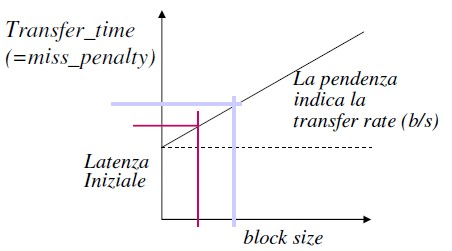
\includegraphics[width=0.5\columnwidth]{img/misspenalty}
\caption{Dipendenza fra tempi di \textit{miss penalty} e grandezza dei blocchi}
\label{fig:misspenalty}
\end{figure}

Compito del saggio e avveduto progettista sarà quindi minimizzare i seguenti parametri (che però sono in dipendenza fra loro!):
\[
T_{Accesso~ medio} = t_{hit} + t_{miss~penalty} \cdot MissRate
\]
\[
t_{miss~penalty} = t_{trasferimento~linea} + PageFaultRate \cdot t_{page~swap}
\]
In queste formule si è fatta l'ipotesi che il tempo di conversione IV -> IF sia incluso in $t_{hit}$, cosa che in realtà non è! Vedremo nel paragrafo \ref{sec:TLB} come è possibile accelerare la traduzione degli indirizzi al fine di raggiungere il miglior risultato possibile in termini prestazionali.

\section{Translation Look-Aside Buffer}
\label{sec:TLB}

Il TLB (\textit{Translation Look-Aside Buffer}) è un elemento fondamentale che ci permette non solo di accelerare la traduzione degli indirizzi, ma anche di gestire un maniera corretta le cosiddette \textit{istruzioni restartable}\footnote{Possiamo distinguere fra due tipi di \textit{interrupt}:
\begin{itemize}
\item \textit{trap}: una volta risolto l'\textit{interrupt} partiamo dall'istruzione successiva;
\item \textit{fault}: una volta risolto l'\textit{interrupt} eseguiamo nuovamente la nostra istruzione ripristinando lo stato.
\end{itemize}
}.
In base al principio di località si può definire il \textit{Working Set} di un programma come l'insieme degli indirizzi ai quali il programma tenderà ad accedere nel prossimo futuro. Il \textit{Working Set} può essere localizzato su un piccolo numero di pagine, spesso accedute per via dell'ormai arcinoto \textit{principio di località}. Il trucco sta quindi nel mantenere in TLB (veloce memoria associativa, vedi paragrafo \ref{sec:cache}, con coppie [nome, valore]) le pagine di questo \textit{Working Set} così da poterle avere a disposizione con grande alacrità.

\begin{figure}[!h]
\centering
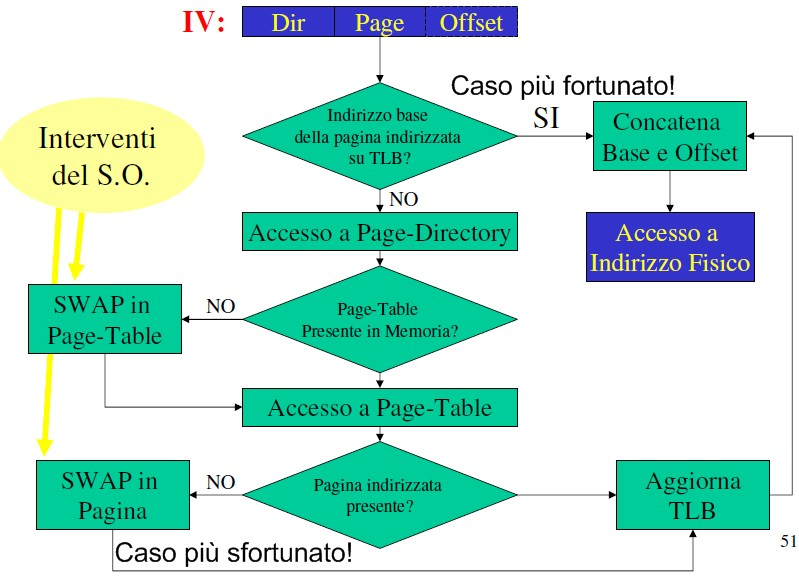
\includegraphics[width=0.9\columnwidth]{img/percorsoTLB}
\caption{Schema di principio dell'accesso a un indirizzo fisico a partire da un indirizzo virtuale}
\label{fig:percorsoTLB}
\end{figure}

Il Processore Pentium dispone di 3 TLB: uno per pagine di codice con 32 elementi (\textit{Page Table Entries}, PTE), uno per pagine di dati di 4 KB con 64 elementi e un ultimo per pagine di dati di 4 MB con 8 elementi.

Ogni \textit{entry} del TLB si riferisce quindi ad una pagina (4 KB), ma come facciamo se per caso cambiamo \textit{task}? In tal caso vengono aggiornati il registro CR3 e la \textit{Page Directory}, cosa che invalida le coppie IV/IF fino a quel momento presenti in TLB: per questo serve effettuare il \textit{flush} (svuotamento) del TLB ad ogni cambio di \textit{task}. In più esiste la possibilità di invalidare una singola \textit{entry} del TLB con l'istruzione INVLPG e di proteggere alcune importantissime pagine (quelle del sistema operativo) dal \textit{flush} settando il bit G nel relativo descrittore.

\section{\textit{Cache} e memorie associative}
\label{sec:cache}

La \textit{cache} si colloca tra la memoria fisica e la CPU e, come nel caso della memoria fisica, anche la \textit{cache} è suddivisa in blocchi di uguale dimensione. Nel caso delle \textit{cache} questi blocchi sono detti \textit{Linee di Cache}. Nel Pentium e nel P6 (bus dati da 64 bit) la dimensione di ogni linea di \textit{cache} è 32 Byte ed è identificabile dai 27 bit BA[31..5] dell'indirizzo fisico (vedi fig. \ref{fig:cache2}).

\begin{figure}[!h]
\centering
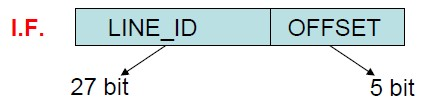
\includegraphics[width=0.35\columnwidth]{img/cache2}
\caption{Indirizzo fisico}
\label{fig:cache2}
\end{figure}

Per il \textit{mapping}, la \textit{cache} può essere organizzata sotto forma di tabella, in modo simile al TLB, e con struttura di\textit{ memoria associativa}.

Tabelle associative sono utilizzate dalla CPU in vari contesti:
\begin{itemize}
\item TLB, per la traduzione IV/IF (stadio IF/MEM);
\item traduzione IF->IC (stadio IF/MEM);
\item Branch Rarget Buffer (BTB), per la predizione dinamica del PC (stadio IF);
\item Reservation Stations (RS) (stadio EX).
\end{itemize}

\begin{figure}[!h]
\centering
\includegraphics[width=0.75\columnwidth]{img/vieset}
\caption{Vie e set}
\label{fig:vieset}
\end{figure}

Ogni elemento della nostra \textit{cache} è associato ad una linea ed è costituito da una terna (\textit{tag} $\to$ vedi figure \ref{fig:tagCache} e \ref{fig:cache2}), stato MESI $\to$ vedi paragrafo \ref{sec:mesi}, contenuto della linea $\to$ 32 Byte).

\begin{figure}[!h]
\centering
\includegraphics[width=0.65\columnwidth]{img/tagCache}
\caption{\textit{Cache}: linee e \textit{tag}}
\label{fig:tagCache}
\end{figure}

Ogni "'blocco'" di elementi (vedi figura \ref{fig:cache2}) presente nella struttura associativa individua una \textit{via}\footnote{Ad ogni via corrisponderà un comparatore per capire quale sia la linea giusta da prendere.}; le vie sono organizzate in \textit{set}: le vie di uno stesso set sono interrogate in parallelo (vedi figura \ref{fig:vieset}). 

\begin{figure}[!h]
\centering
\includegraphics[width=0.85\columnwidth]{img/associatività}
\caption{Diversi tipi di associatività delle \textit{cache}}
\label{fig:associatività}
\end{figure}

La memoria \textit{cache} può essere organizzata secondo tre modelli di associatività, come illustrato in figura \ref{fig:associatività} (sia $n$ il numero di elementi che vogliamo far stare nella \textit{cache}):
\begin{itemize}
\item \textit{fully associative}: in questo caso abbiamo un unico set e $n$ vie (nonché $n$ comparatori per capire quale sia il dato giusto fra tali $n$ vie). Le tabelle \textit{fully associative} prevedono che ogni nuovo elemento (coppia nome-valore) possa essere inserito in qualsiasi posizione della tabella. La ricerca avviene infatti in modo completamente associativo: al momento del recupero di un dato il controllo sul campo nome è eseguito in parallelo su tutti gli elementi della tabella. L'implementazione di questa metodologia richiede un comparatore per ogni posizione della tabella, ma garantisce che il tempo di ricerca sia costante, qualunque sia la posizione del dato cercato;
\item \textit{set associative} a \textit{k} vie: abbiamo $k$ vie e $\dfrac{n}{k}$ set. Ogni dato può essere memorizzato in una precisa posizione in ogni via;
\item \textit{mapping diretto}: abbiamo un'unica \textit{via} e $n$ set. Il \textit{mapping} diretto introduce un vincolo evidente nella collocazione dei dati all'interno della tabella: ogni dato può essere infatti mappato in una sola posizione della tabella.
\end{itemize}

\begin{figure}[!h]
\centering
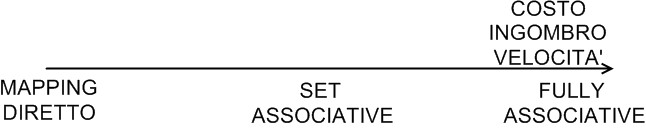
\includegraphics[width=0.75\columnwidth]{img/hitParadeCache}
\caption{Ordinamento dei tre modelli di associatività per costo, velocità e ingombro}
\label{fig:hitParadeCache}
\end{figure}

Qualche osservazione:
\begin{itemize}
\item la dimensione di una \textit{cache} set associative a $K$ vie, con $S$ set per via e $L$ byte per elemento è:
\[ 
Cache ~ Size = S\cdot K \cdot L
\]
\item  a parità di dimensioni della \textit{cache}, se si raddoppiano le vie si dimezzano i set, si riduce di un bit la dimensione dell'indice di set e si aumenta di un bit la dimensione del \textit{tag};
\item  una cache \textit{Fully Associative} altro non è che una \textit{cache} \textit{Set associative} con
S=1;
\item  il numero di vie di una \textit{cache} completamente associativa è:
\[
K =\dfrac{ Cache ~ Size}{L}
\]
\item  nella realizzazione di una \textit{cache} è necessario un comparatore per via; dunque in una \textit{cache} completamente associativa servono $\dfrac{ Cache ~ Size}{L}$ comparatori (tanti quante sono le linee contemporaneamente allocabili in \textit{cache});
\item  la gestione dell'algoritmo LRU in una \textit{cache} completamente associativa è costosa, per cui non viene normalmente applicato.
\end{itemize}

Scendendo nello specifico, ogni via delle \textit{cache} del Pentium è di 4KB, quindi ogni via contiene $2^{12-5}= 128$ linee di \textit{cache}. Una \textit{cache} \textit{set-associative} a 4 vie conterrà 512 linee di \textit{cache}. Se la \textit{cache} ha dimensione opportuna avremo quasi esclusivamente miss \textit{compulsory} (obbligatorie) e la \textit{miss rate} sarà minima.

Nel caso in cui dovesse verificarsi una situazione di \textit{miss} in \textit{cache} (linea di \textit{cache} mancante), il calcolatore deve salire in un livello superiore (memoria fisica), prendere la linea mancante e copiarla in \textit{cache}. Per quest'ultima operazione la CPU ha bisogno del segnale MRDC\# e, dato che ogni linea è di 32 B, abbiamo bisogno di un ciclo di bus con 4 trasferimenti da 64 bit (ciclo \textit{burst}).

\section{Stato MESI}
\label{sec:mesi}

Se abbiamo un sistema \textit{multicore} (e quindi \textit{multimaster}), sarà opportuno che tutti i processori (ognuno dei quali è equipaggiato con una propria \textit{cache}) posseggano per uno stesso dato lo stesso valore: si parla infatti di \textit{cache coherency}. Al fine di garantire la coerenza di \textit{cache} e memoria in un sistema \textit{multimaster} con almeno un \textit{caching agent} è necessario:
\begin{itemize}
\item  definire opportunamente lo stato di ogni linea di \textit{cache};
\item  definire tutti i tipi di accesso che si possono verificare su una linea di \textit{cache};
\item  definire le transizioni di stato e le azioni da svolgere\footnote{Transizioni ed azioni devono essere gestite in hardware in quanto i tempi di attuazione devono essere confrontabili con la durata dei cicli di bus.} ogni volta che viene eseguito un accesso a una linea di \textit{cache}.
\end{itemize}
Nei suddetti sistemi \textit{multimaster} (si noti che anche il semplice Pentium con una CPU e un DMAC è già un sistema \textit{multimaster}!) ogni processore è un \textit{caching agent} e osserva i cicli di bus per scoprire se qualcuno sta accedendo, in lettura o in scrittura, a un dato che è presente nella propria cache (\textit{snooping}): compito di ogni processore è quindi quello di segnalare sul bus il risultato dello \textit{snooping} e di partecipare alla risoluzione della coerenza, affinché all'occorrenza tutti abbiano una copia valida e aggiornata del dato presente in \textit{cache}.
Per coadiuvare e rendere possibile il processo di \textit{cache coherency}, nei processori Intel P5 e P6 si è adottato lo stato MESI (\textit{Modified, Exclusive, Shared, Invalid}); le transizioni e le azioni seguono un insieme di regole sono quindi raggruppate sotto il nome di Protocollo MESI. 

Come abbiamo visto nel paragrafo \ref{sec:cache}, ogni linea di \textit{cache} ha un campo per lo stato MESI: qui si andrà a mettere
\begin{itemize}
\item \textit{invalid} (I): se il dato è invalido. Ci troviamo in questo stato se qualcuno, in giro, ha una versione più aggiornata del dato rispetto a noi;
\item \textit{shared} (S): se stiamo lavorando in politica di \textit{Write True}. Questo significa che il dato in \textit{cache} e quello in memoria sono perfettamente corrispondenti;
\item \textit{exclusive} (E): se stiamo lavorando in politica di \textit{Write Back}, tuttavia vi è corrispondenza fra quanto vi è in \textit{cache} e quanto vi è in memoria;
\item \textit{modified} (M): se lavoriamo in politica di \textit{Write Back}, tuttavia solo la \textit{cache} possiede il dato aggiornato.
\end{itemize}

Andiamo ora a vedere come vengono modificati gli attributi MESI in base a quanto fa la CPU.

\subsection{Accesso in lettura}
\label{sec:accessoLettura}

\begin{figure}[!h]
\centering
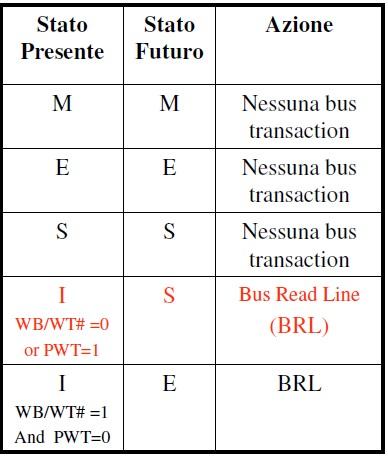
\includegraphics[width=0.35\columnwidth]{img/transLettura}
\caption{Diagramma con transizione degli stati MESI in caso di lettura}
\label{fig:transLettura}
\end{figure}

Stiamo effettuando una LOAD: la CPU è \textit{master}. Come cambiano gli stati?

\begin{itemize}
\item siamo in stato M: questo significa che lavoriamo in politica WB e la \textit{cache} ha il dato aggiornato. Lo stato rimane M perché continuiamo ad avere il dato aggiornato e non compiamo alcun ciclo di bus per reperire alcunché (visto che ne abbiamo la versione più recente);
\item siamo in stato E: lavoriamo in WB e abbiamo corrispondenza fra dato in memoria e dato in\textit{ cache}. Lo stato rimane E perché il dato non ha bisogno di modifiche e non compiamo alcun ciclo di bus per reperire alcunché;
\item siamo in stato S: vi è corrispondenza fra la nostra \textit{cache} e la memoria (o le altre \textit{cache}), quindi non effettuiamo alcun ciclo di bus e usiamo il dato del quale già disponiamo;
\item siamo in stato I: ahia! Il nostro dato è vetusto! A questo punto ciò che accade dipende dalla politica adottata:
\begin{itemize}
\item lavoriamo in WB (WB/WT* = 1): con un ciclo di bus andiamo a reperire la versione aggiornata. Non è però detto che tutti ce l'abbiano: alcuni potrebbero rimandare il suo aggiornamento a quando sarà il loro turno di accedervi. Almeno noi però siamo a posto e mettiamo E;
\item lavoriamo in WT (WB/WT* = 0): a questo punto si innesca il meccanismo che aggiorna il dato facendo sì che abbia lo stesso valore dappertutto. Una volta effettuato il ciclo per portare in \textit{cache} la versione aggiornata, passiamo in S (come vuole la modalità d'uso \textit{Write True}).
\end{itemize}
\end{itemize}

Come si nota, viene generato un ciclo di bus solo in caso di \textit{miss in lettura}, cioè quando scopriamo che il dato nella nostra \textit{cache} è invalido all'atto di volerlo leggere; in questo caso viene generato un ciclo di lettura in memoria (BRL) al quale la memoria risponde anche in caso di \textit{hit} di linea modificata (\textit{hit modified}: "'Ho scoperto che tu ce l'hai aggiornato!'") sulla \textit{cache} di un'altra CPU. In caso di \textit{Hit Modified} il ciclo di lettura viene quindi sospeso e la CPU che contiene il dato modificato farà un ciclo di WB per passarci gli ultimi aggiornamenti dell'informazione da noi richiesta; una volta che ci siamo portati in E o in S (in base alla politica), il ciclo di lettura si concluderà felicemente con il nostro bel dato aggiornato\footnote{E vissero tutti felici e contenti.}.

\subsection{Accesso in scrittura}
\label{sec:accessoScrittura}

\begin{figure}[!h]
\centering
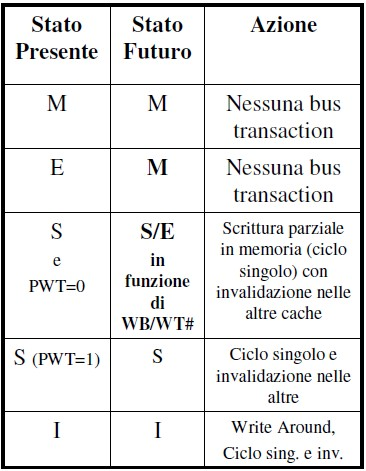
\includegraphics[width=0.35\columnwidth]{img/transScrittura}
\caption{Diagramma con transizione degli stati MESI in caso di scrittura}
\label{fig:transScrittura}
\end{figure}

Stiamo effettuando una STORE (scrittura in memoria). Come cambiano gli stati?
\begin{itemize}
\item siamo in stato M: questo significa che lavoriamo in politica WB e la \textit{cache} ha il dato aggiornato. Ora noi vogliamo ulteriormente scrivere su tale dato aggiornato, cosicché\ldots rimarrà aggiornato (anzi, sarà il più aggiornato!). La scelta è di rimanere in M. Qualcuno potrebbe dire: ma non era meglio andare in E? Non siamo forse i soli ad avere l'ultima versione? Obiezione giusta senonché le altre CPU, molto \textit{voyeur}, si saranno accorte tramite \textit{snooping} che abbiamo scritto una nuova versione del dato e avranno già posto il proprio stato in I (vedi paragrafo \ref{sec:accessoSnooping}). Grazie a questo meccanismo, quindi, noi saremo i soli ad avere M mentre gli altri, aventi tutti I, dovranno prima o poi chiederci le nuove notizie sul dato;
\item siamo in stato E: lavoriamo in WB e abbiamo corrispondenza fra dato in memoria e dato in\textit{ cache}. Abbiamo tuttavia modificato il dato: dovremo giocoforza quindi passare in M;
\item siamo in stato S: fin'ora vi è corrispondenza fra la nostra \textit{cache} e la memoria (o le altre \textit{cache}), 
\begin{itemize}
\item lavoriamo in WB (WB/WT* = 1): il nostro dato è aggiornato e quello degli altri no (siamo in \textit{Write Back} e quindi non glielo passiamo subito): loro si premuniranno di invalidarlo (I) e noi ci fregeremo di essere gli unici ad averlo per il verso (\textit{Exclusive}, E);
\item lavoriamo in WT (WB/WT* = 0): scriviamo il nostro dato in \textit{cache} e poi lo passiamo agli altri; tutti condivideranno (\textit{Share},) quindi automaticamente il dato aggiornato: restiamo in S.
\end{itemize}
\item siamo in stato I: ahia! Il nostro dato è vetusto! A questo punto ciò che accade dipende dalla politica adottata:
\end{itemize}

Ricapitolando: in caso di \textit{miss} si genera un ciclo di bus singolo e la linea resta invalida (politica di \textit{write around}). In caso di \textit{hit} di linea gestita con politica \textit{write through} si genera il ciclo di bus per la scrittura dei soli dati modificati (scrittura parziale) e si chiede l'invalidazione della linea nelle altre \textit{cache} (la linea resta nello stato S). Anche in caso di \textit{hit} di linea potenzialmente condivisa (S) si genera il ciclo di bus per la scrittura dei soli dati modificati (scrittura parziale) e si chiede l'invalidazione della linea nelle altre \textit{cache}. Lo stato della linea può diventare S o E (dipende dal pin WB/WT*). In entrambi i casi la coerenza è assicurata. Gli stati M ed E indicano che la linea è gestita con strategia WB, quindi in questi stati non si generano cicli di bus.

\subsection{Snooping}
\label{sec:accessoSnooping}

\begin{figure}[!h]
\centering
\includegraphics[width=0.75\columnwidth]{img/transSnooping}
\caption{Diagramma con transizione degli stati MESI in caso di \textit{snooping}}
\label{fig:transSnooping}
\end{figure}

Stiamo effettuando lo \textit{snooping}. Come cambiano gli stati? Per questo caso dobbiamo appoggiarci al piedino INV, che è ricavato dall'AND logico fra W/R* e M/IO* (= 1 se qualcuno, diverso da noi, scrivendo in memoria una versione aggiornata del dato). Se il ciclo \textit{snooped} è un ciclo di scrittura (sempre di qualcun'altro, si intende: INV = 1), la linea verrà sempre invalidata perché vorrà dire che il nostro dato non è aggiornato. Se il ciclo \textit{snooped} è di lettura (INV = 0) e la nostra linea è valida, la linea diventerà sempre \textit{shared} (in fin dei conti stiamo condividendo un dato aggiornato con qualcun'altro). Si genera un ciclo di bus solo in caso di \textit{hit} di linea \textit{modified}; questo ciclo si chiama \textit{hit modified writeback cycle}. Si tratta di un ciclo \textit{burst} di scrittura di tutta la linea modificata, inserito in mezzo al ciclo \textit{snooped}; la CPU che aveva generato il ciclo \textit{snooped} dovrà attendere il completamento di questo ciclo di WB per procedere\footnote{L'attesa viene ottenuta mantenendo il segnale di BRDY* non attivo.}.
Quindi:
\begin{itemize}
\item siamo in stato M: questo significa che lavoriamo in politica WB e la \textit{cache} ha il dato aggiornato. 
\begin{itemize}
\item qualcuno sta leggendo quel dato (INV = 0): bloccheremo quel qualcuno perché abbiamo una \textit{hit modified}. Prima che lui possa fare qualsiasi cosa sarà nostra premura passargli il dato aggiornato: dopodiché condivideremo con lui la versione più aggiornata e porremo lo stato ad S;
\item qualcuno sta scrivendo quel dato (INV = 1): idem con patate ma porremo lo stato ad I, visto che quel qualcuno ha ora la versione più aggiornata nella sua \textit{cache}. Beato lui! 
\end{itemize}
\item siamo in stato E: lavoriamo in WB e abbiamo corrispondenza fra dato in memoria (o nelle altre \textit{cache}) e dato nella nostra\textit{ cache}. 
\begin{itemize}
\item qualcuno sta leggendo quel dato (INV = 0): siccome l'età del suo dato è uguale a quello del nostro, passiamo in S perché condividiamo la stessa versione;
\item qualcuno sta scrivendo quel dato (INV = 1): il nostro passerà di moda e metteremo una bella I.
\end{itemize}
\item siamo in stato S: fin'ora vi è corrispondenza fra la nostra \textit{cache} e la memoria (o le altre \textit{cache}),
\begin{itemize}
\item qualcuno sta leggendo quel dato (INV = 0): siccome l'età del suo dato è uguale a quello del nostro, passiamo in S perché condividiamo la stessa versione;
\item qualcuno sta scrivendo quel dato (INV = 1): il nostro passerà di moda e metteremo una bella I; ci aspettiamo tuttavia un rapido e successivo aggiornamento del nostro dato per via della politica \textit{Write True}.
\end{itemize} 
\item siamo in stato I: 
\begin{itemize}
\item qualcuno sta leggendo quel dato (INV = 0): a noi cosa cambia? Indietro eravamo e indietro restiamo;
\item qualcuno sta scrivendo quel dato (INV = 1): idem con patate.
\end{itemize}
\end{itemize}

\begin{figure}[!h]
\centering
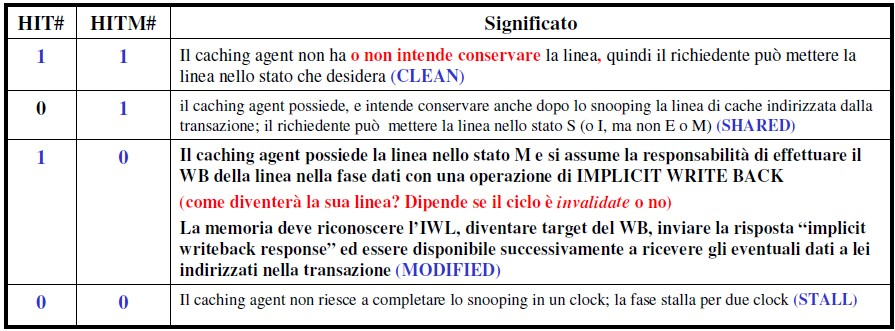
\includegraphics[width=\columnwidth]{img/SegnaliFaseSnooping}
\caption{Alcuni segnali coinvolti nella fase di \textit{snooping}}
\label{fig:SegnaliFaseSnooping}
\end{figure}

\begin{figure}[!h]
\centering
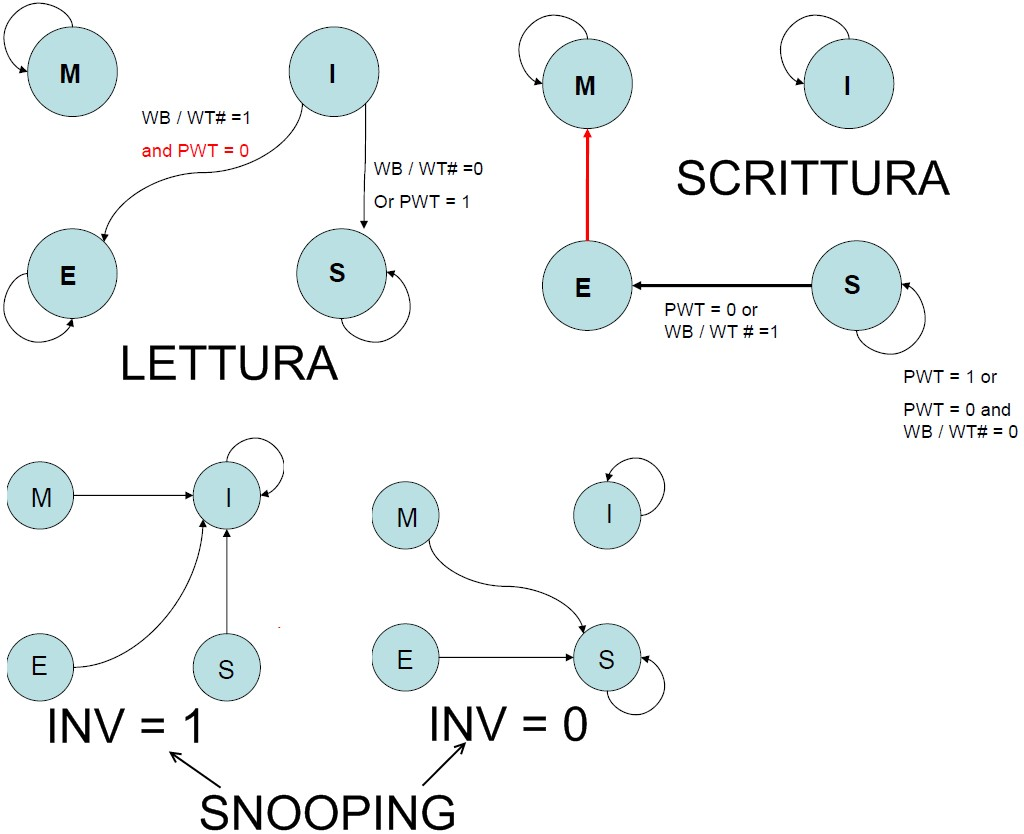
\includegraphics[width=\columnwidth]{img/stateDiagramMESI}
\caption{Riepilogo dei vari diagrammi a stati per il protocollo MESI}
\label{fig:stateDiagramMESI}
\end{figure}
